\documentclass[
	%draft,
	submission,
	%compressed,
	final,
	%
	%technote,
	%internal,
	%submitted,
	%inpress,
	%reprint,
	%
	%titlepage,
	notitlepage,
	%anonymous,
	narroweqnarray,
	inline,
	twoside,
  %invited,
	]{ieee}

\newcommand{\latexiie}{\LaTeX2{\Large$_\varepsilon$}}

%\usepackage{ieeetsp}	% if you want the "trans. sig. pro." style
%\usepackage{ieeetc}	% if you want the "trans. comp." style
%\usepackage{ieeeimtc}	% if you want the IMTC conference style
\usepackage{graphicx}
\usepackage{cite}
\usepackage{url}
\usepackage{amsmath}
\usepackage{placeins}
% Use the `endfloat' package to move figures and tables to the end
% of the paper. Useful for `submission' mode.
%\usepackage {endfloat}

% Use the `times' package to use Helvetica and Times-Roman fonts
% instead of the standard Computer Modern fonts. Useful for the 
% IEEE Computer Society transactions.
%\usepackage{times}
% (Note: If you have the commercial package `mathtime,' (from 
% y&y (http://www.yandy.com), it is much better, but the `times' 
% package works too). So, if you have it...
%\usepackage {mathtime}

% for any plug-in code... insert it here. For example, the CDC style...
%\usepackage{ieeecdc}

\begin{document}

%----------------------------------------------------------------------
% Title Information, Abstract and Keywords
%----------------------------------------------------------------------
\title{Face Obscuration Using Big Data Processing Techniques}

% format author this way for journal articles.
% MAKE SURE THERE ARE NO SPACES BEFORE A \member OR \authorinfo
% COMMAND (this also means `don't break the line before these
% commands).
\author[EILAR AND VENKATESH]{Cody W. Eilar
       \authorinfo{C.\,W.\,Eilar is with the Department of Computer
       Engineering, University of New Mexico, Albuquerque, NM 87109.
       Phone: $+$1\,505\,514-5961, e-mail: ceilar@unm.edu}%
       \and{} Venkatesh Jatla 
       \authorinfo{V.\, Jatla is with the Department of Computer
       Engineering, University of New Mexico, Albuquerque, NM 87109.
       Phone: $+$1\,505\,908-7361, e-mail: venkatesh369@unm.edu}
}

\journal{CS 567, Big Data}
\titletext{ \today \ Dr. Trilce Estrada}
%\ieeecopyright{0018--9456/97\$10.00 \copyright\ 1997 IEEE}
%\lognumber{xxxxxxx}
%\pubitemident{S 0018--9456(97)09426--6}
%\loginfo{Manuscript received September 27, 1997.}
\firstpage{1}

%\confplacedate{Ottawa, Canada, May 19--21, 1997}
\maketitle               

%----------------------------------------------------------------------
% ABSTRACT
%----------------------------------------------------------------------
\begin{abstract} 
  With big data processing techniques and tools becoming ubiquitous, it
  is now more feasible than ever to process images and videos over 
  distributed computing environments using tools such as Hadoop \cite{hadoop}, Spark \cite{spark}, Storm \cite{storm} and others. 

  In this paper, we investigate 
  using these "big-data" techniques to perform face obscuration on very large
  video and image datasets collected by the Advancing Out of School Learning in 
  Mathematics and Engineering (AOLME) program so that these datasets can be 
  safely redistributed. As ulterior motive, we also set in place a frame for
  which we would use to perform other types of detections and activity 
  recognition studies. For the purpose of this paper, we do not use any images
  from the real AOLME dataset, but rather images to illustrate our intention. 
\end{abstract}


%----------------------------------------------------------------------
% SECTION Background and Theory
%----------------------------------------------------------------------
\section{Background}
\PARstart The advancing out of school learning in mathematics and engineering (AOLME) is program designed to help under 
represented middle school students to become interested in science, technology, engineering and mathematics (STEM). The goal of
the program is to not only provide these students with access to high quality programs, but to also help educators analyze
what learning methods work well in the classroom \cite{aolme_paper}. Using video cameras in the classroom, AOLME attempts to capture 
thousands of hours of student to student and student to facilitator interactions. The goal is then to analyze these videos
to further aid educators in understanding what is working in the classroom and what is not, i.e. when students are learning or when they are not. 
The problem with this currently is that
all the videos must be annotated by hand which is very time consuming and tedious. To aid educators with their research, 
it would be extremely useful to have automated methods for annotating videos using machine learning and 
video processing techniques. Because AOLME has a vast array of videos, it seems that "big data" techniques are a
good fit for solving the problem of autonomous video annotation.

The list of potential features that can be extracted from this video data is vast, we
therefore need to narrow the scope of features for
which we can track to a limited subset. Due to restrictions of the IRB, 
it was natural to select features which did not involve the students faces
such as when a student is typing or writing. Since these are the desirable 
features, we no longer needed to have the faces of the students in the videos
and in order to collaborate with other researchers that do not have IRB
approval, we needed a way to remove the faces of the students so that
we could more easily distribute the videos. 

Even with a subset of features, there is still much research to be done
in the fields of activity recognition and motion classification \cite{machine_perception}.
Some research uses action banks \cite{action_bank} which involves
creating very large banks of actions to create feature vectors 
and classify them with support vector machines (SVM). Action banks
can be though of as an extension to object banks. Other techniques involve 
using principal component analysis (PCA) \cite{face_recog_book} to 
detect what features actually contribute to training the classifier.
Regardless of the technique though, there is an obvious need for
research in these fields.

To further this research, we want to make the videos that are available
in the AOLME database more accessible to researchers interested in 
activity recognition and motion classification. In order to do this, 
we need to clean the dataset by removing the faces to satisfy the requirements
of the IRB.

Face recognition is a well studied field because it has applications in 
social media, law enforcement, education, and a myriad of others. There is a 
variety of texts that are available to use as references for this paper such
as \cite{face_recog_book} \cite{kernel_learning} \cite{machine_face_recog} 
as well as many software tools such as OpenCV \cite{opencv} and scikit-image
\cite{scikit-image}. However, the literature in applying these techniques to 
big data limited. Most applications focus on real-time face tracking, or finding
faces in a few hundred images and therefore there is room for research in the area
face detection using big data processing techniques. In this paper, we address 
this topic by looking at using OpenCV, scikit-image, 
Spark and Storm software packages for processing images in very large
video datasets.

The rest of the paper structured as follows: in the theory section we 
present some of the current techniques for facial recognition using 
machine learning to extract features that are necessary for face 
classification. We go over the theory of feature extraction and encoding, 
image-based classifiers, adaptive similarity threshold and temporal filtering. 
In the methodology section, we explain how we can take some of these
techniques and apply them using big data processing techniques. 
We explore experimental set-up and software utilization. It is 
important here that we show how we can leverage existing techniques
to explore some of this large video data effectively using distributed
files systems such as the Hadoop Distributed File System (HDFS) \cite{hadoop}. 
Finally, we explain in the conclusions section how well our 
implementation of face recognition worked with respect to 
performance, accuracy, and feasibility for use with AOLME to
 anonymize the videos for analysis by researchers who do not have
IRB access.  

%----------------------------------------------------------------------
% SECTION THEORY 
%----------------------------------------------------------------------
\section{Theory}
\PARstart As mentioned in the introduction, face detection is a well 
studied field because of all the applications that are involved with 
being able to determine where faces are in data. Face recognition
is nothing more than a subset of a well researched area known as 
pattern recognition. In the subsequent section, we introduce some
of the basic techniques for extracting faces using statistical 
learning theory. Most of the information about this area comes
references \cite{face_recog_book} and \cite{kernel_learning}.
\subsection{Face Detection In Images}
There are many techniques for classifying images such as neural
networks (NN) \cite{face_neural_net}, template matching \cite{face_template}, support vector machines (SVM) \cite{face_svm}, 
nonnegative matrix factorization (NMF) \cite{face_mat_fact}, subspace analysis \cite{face_subspace_analysis}, 
elastic graph matching \cite{face_elastic_bunch}, and finally principal component analysis (PCA) \cite{face_kpca}. 
Though there are many different types of face recognition, in this paper we 
will focus directly on using Eigenfaces, Haar cascasdes, and SVMs. It should be noted 
that some algorithms are very good at determining to whom a face
belongs, but we are only interested in answering the question  
``is this a face?''. In fact, it is more important to uphold the IRB
to have a 100\% accuracy rate at the cost of some false positives.
However, we include eigenfaces in this paper as 
an extension that can be used in later works for those who have IRB approval. 

\subsubsection{Haar Cascades For Face Detection}
Haar Cascades are a well known method in machine learning for rapid object
detection with a high accuracy rate \cite{haar_cascades}. The basic idea
behind the algorithm is that you train the machine with many positive samples
and many negative samples. In our case, we need to train our classifier using
images that contain faces and images that do not. At the heart of the algorithm
is a method of simplifying features instead of using pixel values to classify, 
this is known as an integral image. Equation \ref{eq:integral_image} illustrates
the idea of an integral image. 


\begin{align}
  ii(x,y) = \sum_{x' \leq x, y' \leq y} i(x', y') \label{eq:integral_image}
\end{align}

$x$ and $y$ are the respective columns and rows, and $ii(x,y)$ is the resulting integral
image. This procedure can be done in one pass of the image and greatly reduces
the size of an image. Once the integral image has been determined, we can use
any number of machine learning algorithms to extract the features. In the case of
the Haar Cascades, the \textit{AdaBoost} algorithm was used. We will not go
into the details of that algorithm here. But essentially the \textit{AdaBoos} algorithm 
is designed to select the single rectangle feature which best separates
the positive from the negative samples. A threshold is thus needed $\theta_j$
to determine what amount of misclassification is necessary. 


\begin{equation}
   h_j(x) = \begin{cases}
     1  & \text{if} p_jf_j(x) < p_j \theta_j \\
     0 & otherwise
        \end{cases}
\end{equation}

This classifier is then used at each stage of a cascaded system of classifiers
to reject certain features. For example, if the threshold succeeds for stage one
then it proceeds to the next stage or is immediately rejected. In \cite{haar_cascades}, 
they design each cascade around each convolution kernel shown in Figure 
\ref{fig:haar_cascades}. There would therefore be a total of three stages
or three stages to the cascade shown in Figure \ref{fig:haar_cascades}.

\begin{figure}[h]
\centering
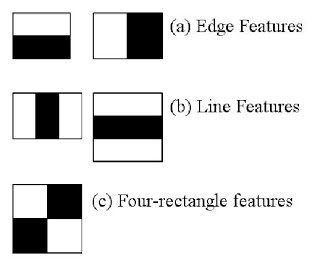
\includegraphics[width=\linewidth]{figures/haar_features}
\caption{Different convolution kernels used on sub-images..}
\label{fig:haar_cascades} 
\end{figure}

Because of their tunable nature, the Haar cascade threshold
can be cranked up to detect 100\% of the faces with some false 
positive rate. This will be especially important for our case
since the data with which we are dealing is sensitive. 

We have now shown that using Haar cascades are ideal for our 
particular case because they are both computationally efficient
making them easy to run on large image sets and can also be 
very accurate in detecting when a face is present. To then remove the face
from the image would then be a trivial task of applying a Gaussian 
blur with a sufficient mean and variance to hide the subjects face 
entirely. Furthermore, 
there are many tools such as OpenCV \cite{opencv} which already have
efficient implementations of this algorithm in both C++ and Python. 


\subsubsection{Eigenfaces for Face Recognition}
Computing the \textit{eigenfaces} is nothing more than using PCA \cite{eigen_faces}. 
The goal with computing the so-called \textit{eigenfaces} is to lower the dimensionality
of an image (or picture) to only its principal components, that is to say
that only relatively small number of dimensions should be used
to sufficiently identify pictures \cite{eigen_faces}. To put this in 
terms of mathematics, we wish to find the eigenvectors of the covariance
matrix for any given set of images \cite{eigen_face_recognition}. To 
illustrate why this is important, if we have a face image that is defined 
as $I(x,y)_{N \times N}$ where $x$ a column, $y$ is a row and $N$ is the
number of rows and columns, an image, for example, that is $256 \times 256$ contains 65,536 elements.
This is to that $I$ has 65,536 dimensions which is a very large number
and not very scalable. Hence PCA or Karhunen-Loeeve expansion is 
applied to find the principle components. These components, or 
eigenvectors coined the name \textit{eigenfaces}. These vectors are thus
used to find the important features in a face image. In order to compute
these vectors, first we
find the average face in a set which is shown in Equation \ref{eq:average_face}

\begin{align}
  \mathbf{\Psi} &= \frac{1}{M} \sum_{n=1}^{M}\Gamma_n \label{eq:average_face}
\end{align}

$\mathbf{\Psi}$ is the average face determined by the total number of faces
in the training set $M$ over all the training images $\Gamma_n$. From 
here we find $M$ orthogonal vectors $\mathbf{u}_n$ and the eigenvalues
$\lambda_k$. Then the vectors $\mathbf{u}_k$ and $\lambda_k$ are the 
eigenvectors and eigenvalues of the covariance matrix show in Equation
\ref{eq:cov_matrix}.


\begin{align}
  C &= \frac{1}{M} \sum_{n=1}^M \mathbf{\Phi}_n \mathbf{\Phi}_n^T \label{eq:cov_matrix} \\
  &= AA^T
\end{align}

Here $\mathbf{\Phi}$ is an $M \times M$ matrix  which is all the 
training faces minus the average of the training faces which is
shown in Equation \ref{eq:subtract_bias}


\begin{align}
  \mathbf{\Phi} &= \Gamma_i - \mathbf{\Psi} \label{eq:subtract_bias}
\end{align}

The covariance matrix shown in equation \ref{eq:cov_matrix} ends up
being an $N^2 \times N^2$ ($N$ is the number of elements in a given 
face image) matrix and finding the eigenvalues for 
this matrix becomes intractable \cite{eigen_face_recognition}. The 
technique to reduce this relies on taking a linear combination of the 
$M \times M$ matrix and using the resulting vectors \cite{turk_eigen_faces}.
From this point, we can now use these \textit{eigenfaces} to classify
a face within an image. The process for doing is the following: 
\begin{itemize}
  \item Receive new face, $\Gamma$ that was not previously seen in the
    training data. 
  \item Project $\Gamma$ into the face space by $\omega_k = \mathbf{u}_k^T (\Gamma - \Psi)$
    for $k = 1 ... M'$ and $M'$ is the number of eigenvectors that are 
    needed to properly classify a face from the input space of $N^2$.
  \item We now have a list, $\omega_k$ of potential matches so now we just need
    to compute the minimum Euclidean distance (or some other any other metric). 
    For example $\epsilon_k = ||\bar{\omega} - \omega_k ||$ where $\bar{\omega}$
    is the mean of the face vectors. 
\end{itemize}

It should also be noted that the above algorithm can be extended to the non-linear
PCA case using the \textit{Kernel Trick} as discussed in \cite{face_kpca}. 
Discussion of the performance of various kernel methods can be found in 
\cite{kernel_learning}.

In this section we have briefly discussed how \texit{eigenfaces} can be
used to recognize a face. This section is not pertinent to face removal, 
but is an extension should we choose to remove only certain faces from 
a scene and not others. 

\subsection{Distributing \textit{Eigenfaces} to Big Data Processes}
Most implementations of face recognition rely on the fact that
all the data is located on one disk and is run on a single machine. 
For this paper, we do not make that assumption and explore the use
of tools such as Spark \cite{spark} and Storm \cite{storm} to create
data that is both resilient and distributed so that many 
calculations can be performed in parallel and collected at the end of a job. 
Figure \ref{fig:distributed_computing_model} 
illustrates our current data structure without the use of any
distributed computing tools.

\begin{figure}[h]
\centering
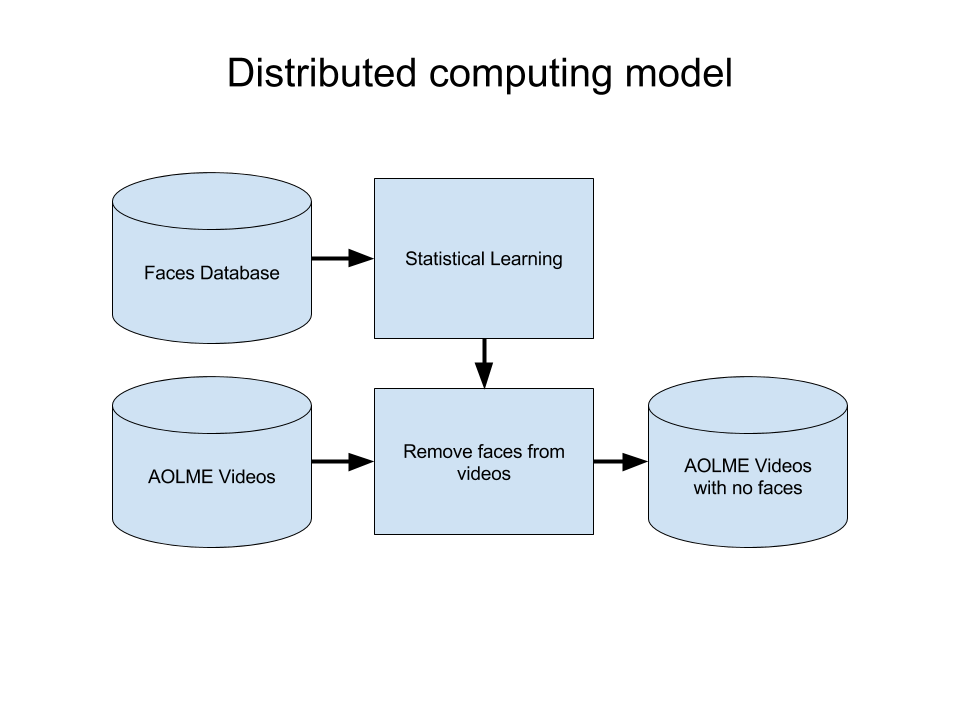
\includegraphics[width=\linewidth]{figures/face_detection_block_diagram}
\caption{Distributed computing model for removing faces from AOLME data.}
\label{fig:distributed_computing_model} 
\end{figure}

\FloatBarrier

The cylindrical shapes shown in Figure \ref{fig:distributed_computing_model}
represent the actual data. In order to construct our statistical learning model,
we need a large database of just faces to create the Haar cascade model
and then from there we can use that model detect the faces in the AOLME
videos. This then would be easily extensible to then determine
which face a given face belongs to. In following sections, we will describe some of the 
fundamental aspects of splitting this diagram up to make use of Spark's
distributed data processing model. 

\subsubsection{Spark: Resilient Distributed Datasets}
Apache Spark is a framework for cluster computing that allows for multi-stage
in-memory processing which in contrast to Hadoop's two-stage MapReduce
framework \cite{spark} \cite{hadoop}. This makes spark ideal for
processing large sets of data quickly, and since it is also built 
on top of Hadoop, can have access to HDFS \cite{spark}. So in order
to leverage this framework, we transform our input data (such as videos
and images) into a format known as a resilient distributed dataset 
or RDD. An RDD is the basic abstraction that the programmer uses
to move data around in a Spark application. It is resilient because
if a single compute node goes down on a distributed network, it does
not stop processing and it is distributed because all the data is 
accessible from every other compute node. This paradigm is illustrated
in Figure \ref{fig:spark_model}.

\begin{figure}[h]
\centering
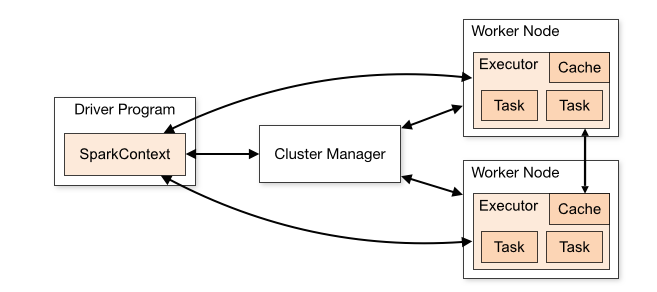
\includegraphics[width=\linewidth]{figures/spark_model}
\caption{Overview of Sparks architecture, image acquired from \cite{spark}.}
\label{fig:spark_model} 
\end{figure}
\FloatBarrier

This paradigm allows us to then have a very large dataset over many compute
nodes and perform facial detection efficiently and reliably to then 
remove faces from the sensitive video data. Future work in this area
could be to us Spark's streaming API to perform near real-time face detection. 
This would then allow us to remove faces in real-time without having to 
modify much of our existing code. 

%----------------------------------------------------------------------
% SECTION METHODOLOGY 
%----------------------------------------------------------------------
\section{Methodology and Experiments} 
\subsection{Machine Learning} 
\subsection{Distributed Computing}

%----------------------------------------------------------------------
% SECTION Conclusion 
%----------------------------------------------------------------------
\section{Conclusion}
\PARstart Conclusion to paper

\bibliography{project.bib}
\bibliographystyle{ieeetr}

\end{document}
